\documentclass{beamer}

\usepackage{Haust2016glærur}

\title{Tölvunarfræði 1a}
\subtitle{Vika 2, seinni fyrirlestur}

\begin{document}

\begin{frame}
\titlepage
\end{frame}

\section{Inngangur}

\begin{frame}{Í síðasta þætti\ldots}
\begin{itemize}
 \item Vigrar og fylki
 \begin{itemize}
  \item Grundvallarnotkun
  \item Víddir fylkja
  \item Fylki og vigrar sem inntök í föll
 \end{itemize}
\end{itemize}
\end{frame}

\section{Aðgerðir á vigra og fylki}

\begin{frame}{Hugtökin}
\begin{columns}
\column{0.5\textwidth}
\begin{itemize}
 \item Vigur: Einvítt safn af stökum, raðað upp í dálk eða línu
 \item Fylki: Tvívítt safn af stökum, raðað upp í flöt
 \begin{itemize}
  \item Líka til útgáfur með fleiri víddum
 \end{itemize}
 \item Skalar: Stakt stak, $1 \times 1$
\end{itemize}
\column{0.5\textwidth}
\begin{center}
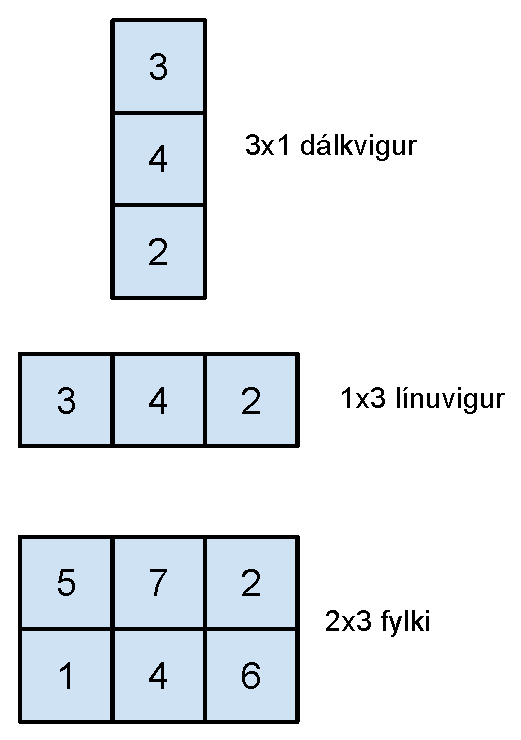
\includegraphics[height=0.8\textheight]{../Pics/vigrar-og-fylki}
\end{center}
\end{columns}
\end{frame}

\subsection{Grundvallaraðgerðir}

\begin{frame}[fragile]{Skalarvirkjar á vigra}
\begin{columns}
\column{0.5\textwidth}
\begin{minted}[frame=lines]{matlab}
>> v = [3 7 2 1];
>> v*3
ans =
    9   21    6    3
>> a = [2 4; 8 6];
>> a/2
ans =
   1   2
   4   3
\end{minted}

\column{0.5\textwidth}
\begin{itemize}
 \item Hægt er að gera skalaraðgerð á öll stök vigurs eða fylkis
 \begin{itemize}
  \item Þ.e.a.s. leggja skalarstærð við öll stök vigurs, margfalda öll stökin með skalarstærð\ldots
 \end{itemize}
 \item Aðgerðinni er þá beitt á hvert stak fyrir sig
 \item Þetta gengur fyrir skalarvirkjana \texttt{+, -, *, /} og \texttt{\textbackslash}
\end{itemize}
\end{columns}
\end{frame}

\begin{frame}[fragile]{Viguraðgerðir}
\begin{columns}
\column{0.5\textwidth}
\begin{itemize}
 \item Aðgerðirnar \texttt{+} og \texttt{-} virka líka á tvo eða fleiri vigra/fylki í einu
 \item Vigrarnir/fylkin þurfa þá að vera af sömu stærð
\end{itemize}

\column{0.5\textwidth}
\begin{minted}[frame=lines]{matlab}
>> v1 = 2:5;
>> v2 = [10, 8, 3, 9];
>> v1+v2
ans =
   12   11    7   14
>> m1 = [1, 2; 3, 4];
>> m2 = [5, 6; 7, 8];
>> m2-m1
ans =
   4   4
   4   4
\end{minted}
\end{columns}
\end{frame}

\begin{frame}{Margföldun og deiling?}
\pause
\begin{columns}
\column{0.5\textwidth}
\begin{itemize}
 \item Línuleg algebra hefur skilgreint aðgerðir sem byggja á margföldun
 \begin{itemize}
  \item \texttt{*}, \texttt{/}, \texttt{\textbackslash} og \texttt{\^}
 \end{itemize}
 \item Það að beita þessum aðgerðum beint á fylki í Matlab hefur sömu áhrif og í línulegri algebru
 \begin{itemize}
  \item Víddir fylkja verða að passa saman
 \end{itemize}
\end{itemize}

\column{0.5\textwidth}
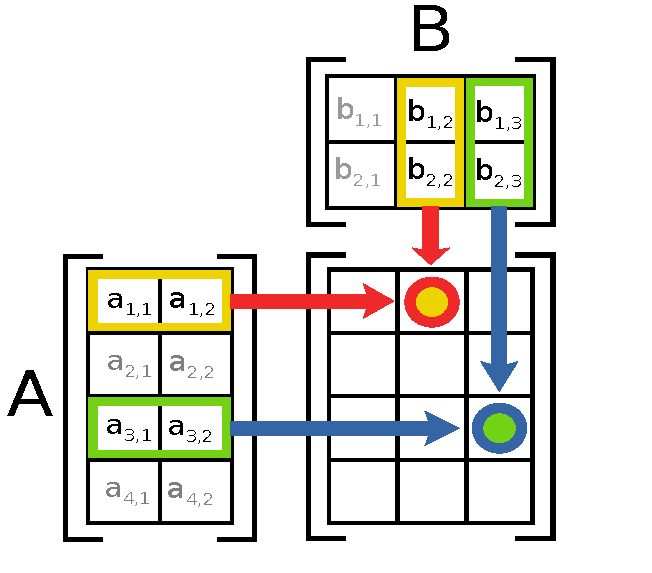
\includegraphics[width=\linewidth]{../Pics/matrix-multiplication}
\end{columns}
\end{frame}

\begin{frame}[fragile]{Fylkjamargföldun í Matlab}
Virkjarnir \texttt{*}, \texttt{/}, \texttt{\textbackslash} og \texttt{\^} framkvæma aðgerðir úr línulegri algebru
\begin{columns}
\column{0.5\textwidth}
\begin{minted}[frame=lines]{matlab}
>> m1 = [0, 1; 2, 3];
>> m2 = [3, 2; 1, 0];
>> m1*m2
ans =
   1   0
   9   4
\end{minted}
\column{0.5\textwidth}
\begin{minted}[frame=lines]{matlab}
>> m1 = randi([0,10],2,3);
>> m2 = randi([0,10],2,3);
>> m1*m2
??? Error using ==> mtimes
Inner matrix dimensions 
must agree.
\end{minted}
\end{columns}
\end{frame}

\begin{frame}[fragile]{Fylkjadeiling}
Hægt er að leysa jöfnuhneppið $A x = b$ með

\begin{minted}[frame=lines]{matlab}
>> x = A\b
\end{minted}

Skilvirkara og nákvæmara er að nota deilingu en að reikna fylkjaandhverfu.
\end{frame}

\begin{frame}[fragile]{Fylkjadeiling}
Dæmi um fylkjadeilingu til að leysa $A x = b$:
\begin{minted}[frame=lines]{matlab}
>> A = [1, 1, 1; 1, 2, 3; 1, 3, 6];
>> b = [3; 1; 4];
>> x = A\b
x =
    10
   -12
     5
\end{minted}
Þetta má svo staðfesta með því að gefa skipunina \texttt{A*x}.

\end{frame}

\begin{frame}[fragile]{Rutt efra stallaform}
Einnig er hægt að leysa jöfnuhneppi með því að nota aukið fylki og \texttt{rref} (reduced row echelon form) fallið:

\begin{minted}[frame=lines]{matlab}
>> rref([A b])
ans =

     1     0     0    10
     0     1     0   -12
     0     0     1     5
\end{minted}

\end{frame}



\begin{frame}[fragile]{Stakvísar fylkjaaðgerðir í Matlab}
\vspace{\baselineskip}
Til að vinna með stök fylkis beint þarf virkjana \texttt{.*}, \texttt{./}, \texttt{.\textbackslash} og \texttt{.\^}
\begin{columns}
\column{0.5\textwidth}
\begin{minted}[frame=lines]{matlab}
>> m1 = [0, 1; 2, 3];
>> m2 = [3, 2; 1, 0];
>> m1.*m2
ans =
   0   2
   2   0
\end{minted}
\column{0.5\textwidth}
\begin{minted}[frame=lines]{matlab}
>> m1 = randi([0,10],2,3);
>> m2 = randi([0,10],2,3);
>> m1.*m2
ans =
   12   30   40
    3   30   60
\end{minted}
\end{columns}
\vspace{\baselineskip}
Ef ætlunin er ekki að stunda línulega algebru, munið eftir punktinum!
\end{frame}

\subsection{Depilfeldi og krossfeldi}

\begin{frame}[fragile]{Depilfeldi}
\begin{columns}
\column{0.4\textwidth}
\begin{itemize}
 \item Hægt er að reikna depilfeldi (e. \emph{dot product}) með vandlegri margföldun eða með \texttt{dot} fallinu
 \item Depilfeldi er skilgreint fyrir tvo jafnstóra vigra
 \begin{itemize}
  \item Ekki skiptir máli hvort um línu- eða dálkvigra er að ræða þegar \texttt{dot} fallið er notað
 \end{itemize}
\end{itemize}
\column{0.6\textwidth}
\begin{minted}[frame=lines]{matlab}
>> c = [3, 5, 2, 4]'; % Dálkvigur
>> r = [2, 8, 1, 4];  % Línuvigur
>> r*c
ans =  64
>> dot(r,c)
ans =  64
\end{minted}
\end{columns}
\end{frame}

\begin{frame}[fragile]{Krossfeldi}
\begin{columns}
\column{0.5\textwidth}
\begin{itemize}
 \item Krossfeldi (e. \emph{cross product}) er skilgreint fyrir 3ja staka vigra
 \begin{itemize}
  \item Úr krossfeldi kemur vigur sem er hornréttur á upphaflegu vigrana
  \item Krossfeldi má reikna út í Matlab með \texttt{cross} fallinu
 \end{itemize}
\end{itemize}
\column{0.5\textwidth}
\begin{minted}[frame=lines]{matlab}
>> v1 = [3, 5, 2];
>> v2 = [2, 8, 1];
>> cross(v1, v2)
ans =
  -11    1   14
\end{minted}
\end{columns}
\end{frame}

\subsection{Yfirlit}

\begin{frame}{Yfirlit viguraðgerða}
\begin{center}
\begin{tabular}{ll}
\toprule
Aðgerð&Merking\\
\midrule
\texttt{A+B}&Stak-fyrir-stak samlagning $A$ og $B$\\
\texttt{A-B}&Stak-fyrir-stak frádráttur $B$ frá $A$\\
\texttt{A.*B}&Stak-fyrir-stak margföldun $A$ og $B$\\
\texttt{A.\^{}B}&Stak-fyrir-stak veldishafning á $A$ með $B$\\
\texttt{A./B}&Stak-fyrir-stak deiling á $A$ með $B$\\
\texttt{A.\textbackslash B}&Stak-fyrir-stak deiling á $B$ með $A$\\
\bottomrule
\end{tabular}
\end{center}
Þessar aðgerðir virka á bæði vigra og önnur fylki
\end{frame}

\begin{frame}{Yfirlit fylkjaaðgerða}
\begin{center}
\begin{tabular}{ll}
\toprule
Aðgerð&Merking\\
\midrule
\texttt{A*B}&Fylkjamargföldun\\
\texttt{A\^{}n}&$A\cdot A\cdot \ldots \cdot A$ (n-sinnum)\\
\texttt{A/B}&Jafngilt  $A\cdot inv(B)$ (þ.e. $AB^{-1}$)\\
\texttt{A\textbackslash B}&Jafngild $inv(A)\cdot B$  (þ.e. $A^{-1}B$)\\
\bottomrule
\end{tabular}
\end{center}
Þessar aðgerðir virka á bæði vigra og önnur fylki
\end{frame}

\begin{frame}{Fyrirlestraræfing}
Skráið ykkur inn á \url{http://socrative.com/} og gerið fyrstu tvær spurningarnar.

Herbergisnúmer = \texttt{TOL105G2016}

Notendanafn = HÍ-tölvupóstfang
\end{frame}

\section{Rökvigrar}

\begin{frame}[fragile]{Rökvigrar}
\vspace{\baselineskip}
Hægt er að framkvæma ýmsar rökaðgerðir á vigra. Niðurstaðan er rökvigur (e. \emph{logical vector}) sem inniheldur sanngildi ($0$ eða $1$) í hverju sæti sínu.
\begin{minted}[frame=lines]{matlab}
>> v = [-4, 2, 0 -1];
>> r = v < 0
r =
   1   0   0   1
\end{minted}
Hér er vigurinn \texttt{v} borinn saman við skalarstærð svo úr verður 4 sæta rökvigurinn \texttt{r}.
\end{frame}

\begin{frame}[fragile]{Rökaðgerðir á fylki}
\vspace{\baselineskip}
Einnig má framkvæma rökaðgerðir á fylki.
\begin{minted}[frame=lines]{matlab}
>> a = randi([0,5],2,4)
a =
   5   5   1   5
   1   0   0   3
>> a == 0
ans =
   0   0   0   0
   0   1   1   0
\end{minted}
\end{frame}

\subsection{Rökvísanir}
\begin{frame}[fragile]{Rökvísanir}
\begin{columns}
\column{0.5\textwidth}
\begin{itemize}
 \item Rökvigur má nota til að framkvæma rökvísun (e. \emph{logical indexing}) í annan vigur
 \item Venjulega er sá vigur sem vísað er í sá vigur sem notaður var til að búa til rökvigurinn til að byrja með
\end{itemize}
\column{0.5\textwidth}
\begin{minted}[frame=lines]{matlab}
>> v = [4, 2, 7, 9, 2];
>> gt5 = v > 5 % Rökvigur
gt5 =
   0   0   1   1   0
>> v(gt5) % Rökvísun
ans =
   7   9
>>  v(v>5) % Styttri leið
ans =
   7   9
\end{minted}
\end{columns}
\end{frame}

\begin{frame}{Rökvísanir vs. ``venjulegar''}
\begin{itemize}
 \item Venjuleg vísun nær í stök eftir númerum
 \begin{itemize}
  \item \texttt{a(2,[1 3]);} nær í stökin í línu 2 og dálkum 1 og 3
 \end{itemize}
 \item Rökvísun nær í þau stök sem svara til sanngilda, eftir staðsetningu
 \begin{itemize}
  \item \texttt{v(logical([0 1 1 0 1]))} nær í stökin í sætum 2, 3 og 5
 \end{itemize}
\end{itemize}
\end{frame}

\begin{frame}[fragile]{Rökvísanir og fylki}
\begin{columns}
\column{0.5\textwidth}
\begin{itemize}
 \item Munum að ekki er hægt að eyða stökum úr ``miðju fylki''
 \begin{itemize}
  \item Fylki þarf alltaf að hafa jafn mörg stök í hverri röð og í hverjum dálki
 \end{itemize}
 \item Þegar rökvísun er beitt á fylki fáum við stökin sem samsvara sönnu gildunum í dálkvigri.
\end{itemize}
\column{0.5\textwidth}
\begin{minted}[frame=single]{matlab}
>> a = [1, 2; 3, 4];
>> a(a ~= 2)
ans =
   1
   3
   4
\end{minted}
\end{columns}
\end{frame}

\begin{frame}{Að búa til rökvigur}
\begin{itemize}
 \item Út frá samanburði við vigur
 \begin{itemize}
  \item \texttt{rv = v > 5;}
 \end{itemize}
 \item Með því að nota \texttt{logical} fallið, sem breytir tölum öðrum en 0 í ``satt'' og 0 í ``ósatt''
 \begin{itemize}
  \item Föllin \texttt{zeros} eða \texttt{ones} geta hér verið mjög gagnleg
  \item \texttt{rv = logical(zeros(1,5));}
 \end{itemize}
 \item Með því að nota föllin \texttt{true} eða \texttt{false}
 \begin{itemize}
  \item \texttt{rv = true(2,2);} býr til $2 \times 2$ fylki með gildunum ``satt''
 \end{itemize}
\end{itemize}
\end{frame}

\subsection{Rökvigrar, föll og virkjar}
\begin{frame}[fragile]{Föll sem vinna með rökvigra}
\begin{columns}
\column{0.5\textwidth}
\begin{itemize}
 \item Matlab hefur þó nokkur innbyggð föll sem hægt er að nota á rökvigra
 \begin{itemize}
  \item \texttt{any} skilar satt ef einhver stök vigursins eru ekki $0$
  \item \texttt{all} skilar satt ef öll stök vigursins eru ekki $0$
  \item \texttt{not} snýr við sanngildi vigurs
  \item Einnig: \texttt{find}
 \end{itemize}
\end{itemize}
\column{0.5\textwidth}
\begin{minted}[frame=single]{matlab}
>> v = 1:5;
>> rv = v > 2
rv =
   0   0   1   1   1
>> any(rv)
ans =  1
>> all(rv)
ans = 0
\end{minted}
\end{columns}
\end{frame}

\begin{frame}[fragile]{Fallið find}
Fallið \texttt{find} skilar sætisnúmerum þeirra staka í vigri sem ekki eru 0. Venjulega er það notað á rökvigra.
\begin{minted}[frame=single]{matlab}
>> v = [5, 0, -1, 3, 8];
>> find(v) % Hvaða stök v eru ekki 0?
ans =
   1   3   4   5
>> find(v>2) % find beitt á rökvigur
ans =
   1   4   5
\end{minted}
\end{frame}

\begin{frame}[fragile]{Rökvirkjarnir |, \& og \~{}}
\vspace{\baselineskip}
\begin{columns}
\column{0.5\textwidth}
\begin{itemize}
 \item Rökvirkjarnir |, \& og \~{} vinna stak-fyrir-stak á vigrum
 \begin{itemize}
  \item Getum beitt þeim á rökvigra
 \end{itemize}
 \item Rökvirkjarnir \texttt{||} og \texttt{\&\&} virka á skalarstærðir
 \begin{itemize}
  \item Tilraunir til að nota skalar-virkjana á vigra eða öfugt eru líklegar til að gefa óvæntar niðurstöður
 \end{itemize}
\end{itemize}
\column{0.5\textwidth}
\begin{minted}[frame=single]{matlab}
>> rv1 = logical([1, 0]);
>> rv2 = logical([1, 1]);
>> rv1 & rv2
ans =
   1   0
>> rv1 | rv2
ans =
   1   1
>> ~rv1
ans =
   0   1
\end{minted}
\end{columns}
\end{frame}

\begin{frame}{Fyrirlestraræfing}
Skráið ykkur inn á \url{http://socrative.com/} og gerið seinni þrjár spurningarnar.

Herbergisnúmer = \texttt{TOL105G2016}

Notendanafn = HÍ-tölvupóstfang
\end{frame}


\end{document}
